\section{Nonce Reuse on Sensors}\label{sec:nonce}

Every signature of the repaired scheme uses a fresh random nonce $t_i$, and the paper only states that
$t_i$ is chosen uniformly at random~\cite{qiao2023}. Sensors are where randomness fails in practice: a
generator stuck or re-seeded after a reboot, a firmware or virtual-machine image cloned together with its
seed, or too little entropy at boot. We asked what a repeated nonce costs.

\subsection{Key recovery}
The attack is the standard nonce-reuse attack on Schnorr-type signatures; our contribution is working it
out for this scheme. From \cref{eq:qiao-sign}, $z_i=t_i+c_iu_i+sk_iv_i$, where $u_i$ and $v_i$ are hashes
of public data. Every signature made under the same nonce $t$ is one more linear equation in the same
unknowns, and the repetition is visible because the same commitment $T=tP$ appears in each signature.

How many signatures are needed depends on the scheme and the attacker (\cref{tab:nonce}). In Verma's
scheme the certificate term $c_i$ has coefficient 1, so the nonce and the certificate merge into one
unknown and two signatures reveal $sk_i$ (although Verma's scheme is forgeable with none,
\cref{sec:keyonly}). The repair multiplies $c_i$ by the per-message hash $u_i$, which makes it a separate
unknown: an outsider needs three signatures and solves a $3\times3$ linear system for $t$, $c_i$ and $sk_i$
(\cref{app:nonce}). With only two signatures, every guess of $sk_i$ fits some $c_i$, and picking the right
one is as hard as a discrete logarithm. The KGC, however, issued the certificate and already knows $c_i$,
so two signatures give it $sk_i$, the very key that certificate-based signatures promise the KGC never
learns.

\begin{table}[ht]
\centering\small
\caption{Signatures under one nonce needed to recover the signer's secrets (8 trials each).}\label{tab:nonce}
\begin{tabular}{llcl}
\toprule
Scheme and attacker & Unknowns & Signatures & Result \\
\midrule
Verma, anyone & $sk_i$ and $r_{2i}+c_i$ (merged) & 2 & secret key recovered, 8/8 \\
Repaired, outsider & $t$, $c_i$, $sk_i$ & 3 & both secrets recovered, 8/8 \\
Repaired, the KGC & $t$, $sk_i$ (knows $c_i$) & 2 & $sk_i$ recovered, 8/8 \\
Repaired, hedged nonce & no shared nonce & --- & attack cannot start, 8/8 \\
\bottomrule
\end{tabular}
\end{table}

The recovered keys are checked against $pk_i$ and the certificate equation before use. With them the
attacker signs a message of its choice with a fresh nonce; the forgery verifies (8/8) and passes
aggregate verification next to honest signatures (8/8). The server sees only valid signatures throughout
(\cref{fig:nonce}).

\begin{figure}[ht]
\centering
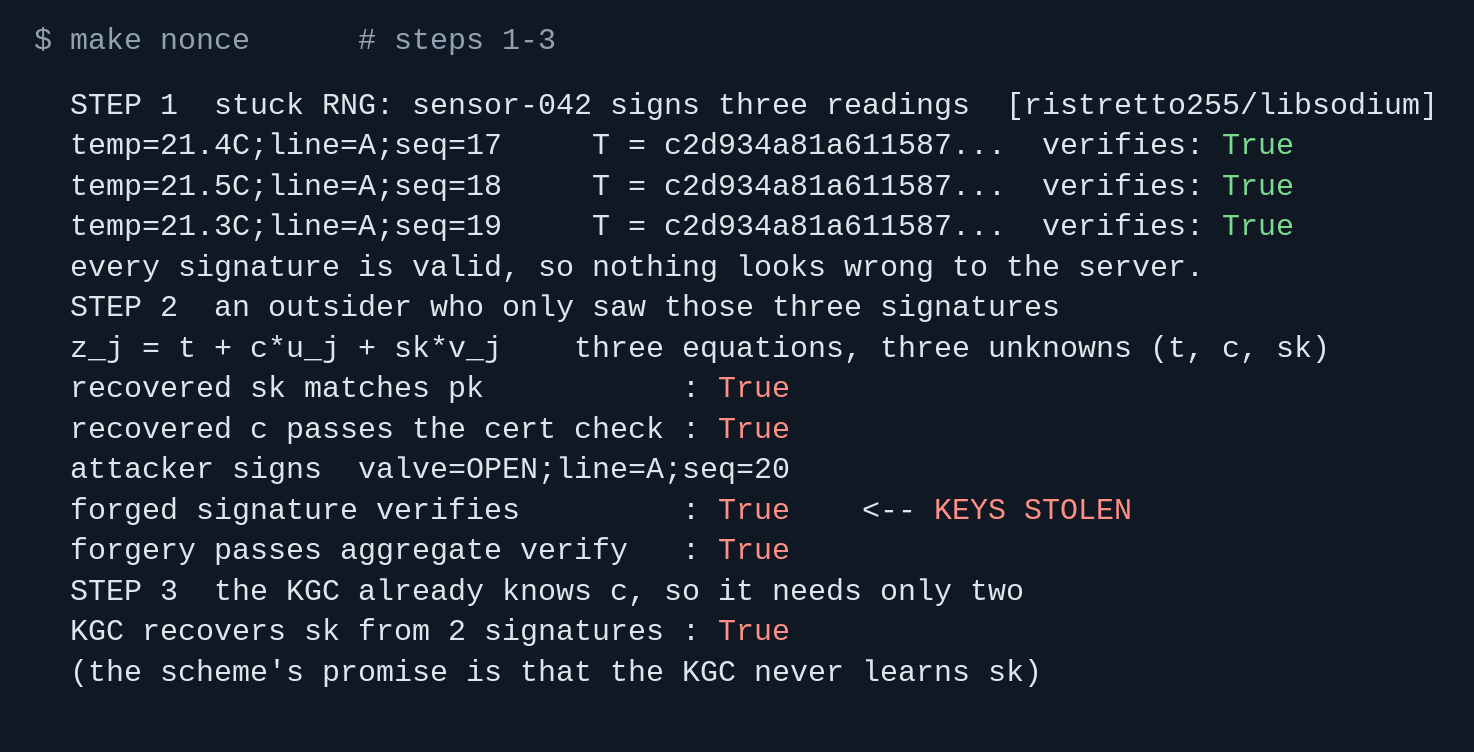
\includegraphics[width=0.9\linewidth]{figures/final_demo2_attack.png}
\caption{Captured output of \code{make nonce}: three readings signed under a stuck generator share one
$T$ and all verify; an outsider recovers both secrets and signs \code{valve=OPEN}; the KGC needs only two
signatures.}\label{fig:nonce}
\end{figure}

\subsection{The fix: a hedged nonce}
\prov{Implementation}, using a standard technique~\cite{rfc6979,rfc8032}. Instead of taking the nonce
straight from the generator, the signer derives it from its secrets and the message and mixes in the
generator's output:
\begin{equation}
t_i=H_{\mathrm{nonce}}(sk_i,\ c_i,\ m_i,\ pk_i,\ R_i,\ id_i,\ \Delta,\ \text{fresh randomness}).
\end{equation}
The secrets keep the nonce unpredictable, the message makes different messages get different nonces even
when the generator is stuck, and the fresh randomness keeps a working generator useful against fault
attacks on purely deterministic nonces. The signing equation and the signature format are unchanged, so
every existing verifier accepts hedged signatures, also in aggregates mixed with ordinary ones. With the
generator stuck, the three nonces were distinct in 8 of 8 trials, all signatures verified, and the
recovery attack could not start. The paper specifies no nonce derivation at all.
